%!TEX root = ../template.tex
\chapter{Designing a DSL in Rust (10/02/2021)}\label{cha:rust-dsl}

\section{Rust Macros}

Just like its predecessors, C \& C++, Rust offers macros as part of the language.
In essence, Rust macros are just like other languages macro's, they generate code before compilation.
In Rust, macros refer to a family of features (see \autoref{fig:rust-macro-family}),
\emph{declarative} macros and \emph{procedural} macros.

\begin{figure}
    \centering
    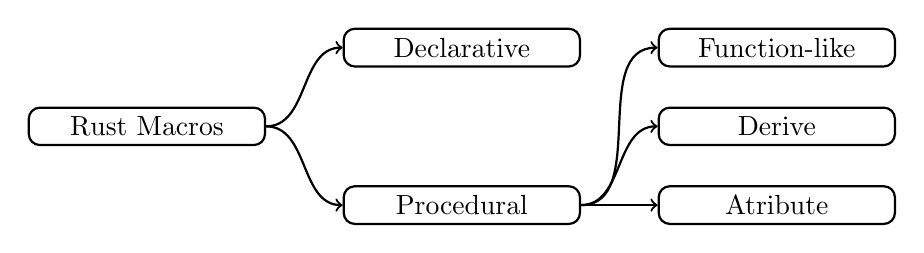
\begin{tikzpicture}
        \tikzset{
            member/.style={
                rectangle,
                rounded corners,
                draw=black,
                thick,
                minimum width=3cm,
            },
            connection/.style={->, thick},
        }
        % \draw (0, -2) grid (6, 2);
        \node[member] (root) at (-1, 0) {Rust Macros};
        \node[member] (decl) at (3, 1) {Declarative};
        \node[member] (proc) at (3, -1) {Procedural};
        \node[member] (func) at (7, 1) {Function-like};
        \node[member] (derv) at (7, 0) {Derive};
        \node[member] (attr) at (7, -1) {Atribute};
        \draw[connection] (root) edge[out=0, in=180] (proc);
        \draw[connection] (root) edge[out=0, in=180] (decl);
        \draw[connection] (proc) edge[out=0, in=180] (func);
        \draw[connection] (proc) edge[out=0, in=180] (derv);
        \draw[connection] (proc) edge[out=0, in=180] (attr);
    \end{tikzpicture}
    \caption{Rust macro's family tree}
    \label{fig:rust-macro-family}
\end{figure}

\subsection{Declarative Macros}

Declarative macros are also known as \emph{macros-by-example}, they can be declared with \texttt{macro\_rules!}
and are called with function syntax (see \autoref{lst:rust-macro-rules}).
% These macros work by pattern matching, supporting several kinds of \emph{metavariables},
% they also support matching repeating patterns and
% TODO stolen from https://doc.rust-lang.org/reference/macros-by-example.html
Each macro by example has a name, and one or more rules. Each rule has two parts:
a matcher, describing the syntax that it matches, and a transcriber,
describing the syntax that will replace a successfully matched invocation.
Both the matcher and the transcriber must be surrounded by delimiters.
Macros can expand to expressions, statements, items (including traits, impls, and foreign items), types, or patterns.

\paragraph{Transcribing.}%
% TODO stolen from https://doc.rust-lang.org/reference/macros-by-example.html#transcribing
When a macro is invoked, the macro expander looks up macro invocations by name, and tries each macro rule in turn.
It transcribes the first successful match; if this results in an error,
then future matches are not tried. When matching, no lookahead is performed;
if the compiler cannot unambiguously determine how to parse the macro invocation one token at a time, then it is an error.

\paragraph{Metavariables.}%
To specify a macro a user first declares a pattern which will match a given form of syntax.
\emph{Metavariables} are used to achieve such goal,
they are declared with “\texttt{\$ \keyword{name} : \keyword{fragment-specifier}}” in the macro matcher and
can match thirteen different kinds of syntax fragments.
% TODO add link to https://doc.rust-lang.org/reference/macros-by-example.html#metavariables
In \autoref{lst:rust-macro-rules}, the metavariable \texttt{n} is of kind \texttt{literal}
which will match literals such as \texttt{'c'}, \texttt{"String"} and \texttt{1337}.
% TODO add link to https://doc.rust-lang.org/reference/expressions/literal-expr.html

\paragraph{Repetitions.}%
Repetitions are indicated by placing the tokens to be repeated inside \texttt{\$(...)},
followed by a repetition operator, optionally with a separator token between.
This is valid both for the matcher and the transcriber.
Repetition operators are the same as the regular expression ones:
\begin{compactitem}
    \item \texttt{*} — indicates zero or more repetitions.
    \item \texttt{+} — indicates at least one repetition.
    \item \texttt{?} — indicates zero or one repetition.
\end{compactitem}

\paragraph{Hygiene.}%
% TODO add link https://veykril.github.io/tlborm/macros/minutiae/hygiene.html
Declarative macros are \emph{partially} hygienic, meaning they are hygienic when it comes to most identifiers,
but not when it comes to generic type parameters or lifetimes.
Hygiene works by attaching an invisible "syntax context" value to all identifiers. When two identifiers are compared,
both the identifiers' textural names and syntax contexts must be identical for the two to be considered equal.

\begin{listing}
    \centering
    \begin{minted}{Rust}
macro_rules! say_hello {
    ($n:literal) => {
        for 0..$n {
            println!("Hello, world!");
        }
    }
}
fn main() {
    say_hello!(5);
}
    \end{minted}
    \caption{Example \texttt{macro\_rules!} usage.
        When executed, the code above will print “\texttt{Hello, world!}” five times.}
    \label{lst:rust-macro-rules}
\end{listing}

\begin{listing}
    \centering
    \begin{minipage}[t]{0.45\textwidth}
        \begin{minted}{Rust}
macro_rules! using_a {
    ($e:expr) => {
        {
            let a = 42;
            $e
        }
    }
}
let four = using_a!(a / 10);
    \end{minted}
        \subcaption{\texttt{using\_a} macro definition.}
        \label{lst:rust-macro-hygiene:a}
    \end{minipage}
    \hspace{2mm}
    \begin{minipage}[t]{0.45\textwidth}
            \begin{minted}[
                numbers=right,
                highlightlines=2,
                highlightcolor=blue!10
            ]{Rust}
let four = {
    let a = 42;
    a / 10
};
        \end{minted}
        \subcaption{\texttt{using\_a} macro expansion.
        Declarations with a blue background will be placed in a different \emph{scope} than the others.}
        \label{lst:rust-macro-hygiene:b}
    \end{minipage}%
    \caption{Hygienic macro expansion.}
    \label{lst:rust-macro-hygiene}
\end{listing}

% TODO add more text
% TODO add references to the reference

\subsection{Procedural Macros}

Rust also has another macro mechanism, \emph{procedural macros},
these can take three forms: \emph{function-like macros}, \emph{derive macros} and \emph{attribute macros}.
In a nutshell, procedural macros allow users to run code at compile time, consuming and producing Rust syntax.


\subsubsection*{Function-like}

\subsubsection*{Derive}
Derive macros likely are the most common kind of procedural macro in Rust,
they are usually used to \emph{derive} a \keyword{trait} implementation from a \keyword{struct} (see \autoref{lst:rust-derive-debug}).
They define new inputs for the \texttt{derive} attribute,
and can also create new items given the token stream of a \keyword{struct}, \keyword{enum} or \keyword{union}.

\paragraph{Definition.}%
Derive macros are defined as public functions with the \texttt{proc\_macro\_derive} attribute
and a signature of \texttt{(TokenStream) -> TokenStream}.
The input is a token stream of the item with the \texttt{derive} attribute,
the output is a set of items that are appended to the module or block where the input token stream is in.
In \autoref{lst:rust-derive-debug} the \keyword{Debug} implementation will be appended to the end of the structure.

\paragraph{Helper Attributes.}%
Derive macros are also able to add additional attributes to the scope of the current item.
Such attributes are called \emph{derive macro helper attributes} and they are \emph{inert},
that is, they are not processed by themselves but rather serve as annotations (see \autoref{lst:rust-derive-error}).

\subsubsection*{Hygiene}
In contrast with \texttt{macro\_rules!}, procedural macros are \emph{unhygienic},
meaning their output can interfere with the surrounding code and vice-versa,
like C macros, they act as if the output code was simply written in the original source file.
This leads developers to be required to add a series of extra measures when outputting code
such as using absolute paths and function names which are unlikely of clashing with user code.
% TODO add Koriaxet guide here

\begin{listing}
    \centering
    \begin{minted}{Rust}
#[derive(Debug)]
struct Coordinate {
    x: f32,
    y: f32,
    x: f32,
}
    \end{minted}
    \caption{
        Example usage of \keyword{\#[derive(...)]},
        in this case deriving \keyword{Debug} enables the structure to be printed with
        “\mintinline{Rust}{println!("{:?}", coord)}”.
    }
    \label{lst:rust-derive-debug}
\end{listing}

\begin{listing}
    \centering
    \begin{minted}{Rust}
#[derive(Error)]
enum CoordinateError {
    #[error("Invalid coordinates {0}")]
    InvalidCoordinates(Coordinates),
}
    \end{minted}
    \caption{
        Example usage of a derive macro with helper attributes,
        in this case the \texttt{error(...)} defines an error message with a \texttt{Coordinates} parameter.
    }
    \label{lst:rust-derive-error}
\end{listing}

\subsubsection*{Attribute}

\section{The DSL}
\subsection{Objectives}
What the DSL should achieve
\subsection{Architecture}
How it achieves it